% arara: lualatex
\chapter[Dielectric surface loss in superconducting resonators with flux-trapping holes]{Dielectric surface loss in superconducting resonators with flux-trapping holes\footnote{This chapter was published as: "Dielectric surface loss in superconducting resonators with flux-trapping holes",  B. Chiaro, et al. SUST \textbf{29}, 10 (2016)}}
\label{ch:vortex}


%\begin{document}
\def \Bcapp {\text{B}^{\textrm{cool}}_{\textrm{applied}}}
\def \Qtlsparticipation {1/Q_{\text{TLS}} = \Sigma_{i}\, p_i \tan \delta_i}

\begin{comment}
\preprint{}

\title{Dielectric surface loss in superconducting resonators with flux-trapping holes}

\author{B. Chiaro}
\affiliation{Department of Physics, University of California, Santa Barbara, California 93106, USA}
\author{A. Megrant}
\affiliation{Department of Physics, University of California, Santa Barbara, California 93106, USA}
\affiliation{Department of Materials, University of California, Santa Barbara, California 93106, USA}
\author{A. Dunsworth}
\affiliation{Department of Physics, University of California, Santa Barbara, California 93106, USA}
\author{Z. Chen}
\affiliation{Department of Physics, University of California, Santa Barbara, California 93106, USA}
\author{R. Barends}
\affiliation{Google Inc., Santa Barbara, California 93117, USA}
\author{B. Campbell}
\affiliation{Department of Physics, University of California, Santa Barbara, California 93106, USA}
\author{Y. Chen}
\affiliation{Google Inc., Santa Barbara, California 93117, USA}
\author{A. Fowler}
\affiliation{Google Inc., Santa Barbara, California 93117, USA}
\author{I.C. Hoi}
\affiliation{Department of Physics, University of California, Santa Barbara, California 93106, USA}
\author{E. Jeffrey}
\affiliation{Google Inc., Santa Barbara, California 93117, USA}
\author{J. Kelly}
\affiliation{Google Inc., Santa Barbara, California 93117, USA}
\author{J. Mutus}
\affiliation{Google Inc., Santa Barbara, California 93117, USA}
\author{C. Neill}
\affiliation{Department of Physics, University of California, Santa Barbara, California 93106, USA}
\author{P. J. J. O'Malley}
\affiliation{Department of Physics, University of California, Santa Barbara, California 93106, USA}
\author{C. Quintana}
\affiliation{Department of Physics, University of California, Santa Barbara, California 93106, USA}
\author{P. Roushan}
\affiliation{Google Inc., Santa Barbara, California 93117, USA}
\author{D. Sank}
\affiliation{Google Inc., Santa Barbara, California 93117, USA}
\author{A. Vainsencher}
\affiliation{Department of Physics, University of California, Santa Barbara, California 93106, USA}
\author{J. Wenner}
\affiliation{Department of Physics, University of California, Santa Barbara, California 93106, USA}
\author{T. C. White}
\affiliation{Department of Physics, University of California, Santa Barbara, California 93106, USA}
\author{John M. Martinis}

\affiliation{Department of Physics, University of California, Santa Barbara, California 93106, USA}
\affiliation{Google Inc., Santa Barbara, California 93117, USA}

\date{\today}

\begin{abstract}

Surface distributions of two level system (TLS) defects and magnetic vortices are limiting dissipation sources in superconducting quantum circuits.  Arrays of flux-trapping holes are commonly used to eliminate loss due to magnetic vortices, but may increase dielectric TLS loss.  We find that dielectric TLS loss increases by approximately 25\,\% for resonators with a hole array beginning 2\,$\mu \text{m}$ from the resonator edge, while the dielectric loss added by holes further away was below measurement sensitivity.  Other forms of loss were not affected by the holes.  Additionally, we estimate the loss due to residual magnetic effects to be \mbox{$9\times 10^{-10} /\mu\text{T} $} for resonators patterned with flux-traps and operated in magnetic fields up to $5$\,$\mu\text{T}$.  This is orders of magnitude below the total loss of the best superconducting coplanar waveguide resonators.

\end{abstract}
\maketitle
\end{comment}

Superconducting coplanar waveguide (SCPW) resonators are extensively used in astronomy\cite{day2003,mazin2012} and quantum information \cite{mariantoni2011,barends2013,jeffrey2014}.  An important frontier in SCPW resonator development is increasing the intrinsic quality factor $Q_i = 1/\text{loss}$.  This is an especially important proxy for qubit performance, since the resonator $Q_i$ is strongly correlated with the qubit relaxation time $T_1$ because qubits and resonators are subject to many of the same dissipation mechanisms.\cite{wang2015, wisbey2010, song2009a, wang2014, nsanzineza2014, martinis2005, martinis2009, gao2008}  Quantum computers require low operating temperatures $\lesssim 100\,\textrm{mK}$, single-photon excitation energies, low magnetic fields $\lesssim 5\mu\textrm{T}$, and high coherence  $Q_i \gtrsim 10^{6}$.  In this quantum computing regime, dominant loss mechanisms are two-level state (TLS) defects in amorphous dielectrics located at surfaces and loss from trapped flux in magnetic vortices.

In this Letter, we examine the tradeoff between increased TLS loss and reduced magnetic vortex loss that occurs when the ground plane of SCPW resonators is patterned with an array of holes.  Fractal resonators also reduce magnetic losses, but are typically optimized for use in high magnetic fields and have not demonstrated quality factors as high as coplanar designs in small field environments.\cite{graaf2012}  Although hole arrays have long been known to eliminate dissipation from trapped flux, \cite{song2009b, bothner2011, bothner2012} these structures have not been studied in the quantum computing regime for the possibility of increasing TLS loss. Our data shows that dielectric TLS loss from flux-trapping holes is an important physical limitation if designed incorrectly.   

When a thin-film superconductor is cooled through its transition temperature $T_c$ in a magnetic field $B_{\textrm{cool}}$, it is energetically favorable for magnetic flux to be trapped as vortices at some defect\cite{stan2004}.  The typical spacing between vortices or an edge of the superconducting film to a vortex is $\left( \Phi_{0} / B_{\textrm{cool}} \right)^{1/2}$. As the superconducting order parameter has to vanish\cite{tinkham}, this normal core produces dissipation in response to currents flowing past the core\cite{song2009a}.  With a hole in the film, vortices form without a normal core and produce no dissipation.  We note that suitably positioned normal-core vortices may be beneficial as quasiparticle traps\cite{nsanzineza2014,wang2014}.  For this application, hole arrays should be positioned properly to engineer the number and position of the normal-core vortices. 

Because the holes have sharp edges and expose the substrate, they introduce new dissipation sites from surface TLS defects.  As modern high-$Q$ resonators are sensitive to  nanometer thick amorphous dielectrics at surfaces\cite{wenner2011}, these additional edges can increase loss if the holes are placed near the resonator where the electric fields are the largest.  Consequently, we must determine how closely holes can be safely placed from the resonator.

We characterize this loss with quarter-wavelength SCPW resonators that are capacitively coupled to a feedline, with frequency multiplexing to measure 10 resonators per chip.  An optical image of a device wirebonded in a mount is shown in Fig.\,\ref{Schematic}(a). The resonators have fundamental frequencies between 4.6\,GHz and 5.5\,GHz and center trace and gap dimensions of $15\,\mu\text{m}$ and $10\,\mu\text{m}$.  Our circuit contains both resonators with and without ground-plane holes for direct comparison.  Our arrays are made from square holes of side length $2\,\mu\text{m}$ and an edge to edge separation $d$ of $2\,\mu \text{m}$, $6\,\mu \text{m}$, or $10\,\mu \text{m}$.  The distance $d$ is also the distance between the edge of the resonator gap and the nearest hole.  An example is shown in Fig.\,\ref{Schematic}(b).  The equivalent circuit diagram for this device near resonance is shown in Fig.\,\ref{Schematic}(c) and was analysed in detail in Ref.% TODO \,\onlinecite{megrant2012}.

Our resonator circuits were fabricated from 100\,nm aluminium thin films grown on c-plane sapphire substrates. The first type is made in a conventional electron beam deposition system with base pressure of $~3\times 10^{-8}\,\textrm{Torr}$.  Films from this tool yield resonators with $Q_i \simeq 8 \times 10^{5}$ near a measurement photon number $N_\textrm{photon} = 1$ and are thus representative of resonators made with standard deposition techniques.  The second type was prepared in a molecular beam epitaxy (MBE) system with a base pressure of $~ 1\times 10^{-11}\,\textrm{Torr}$.  With an in-situ $\text{O}_2$ plasma cleaning of the substrate at $650$\,$^\circ$C \cite{megrant2012}, we found lower resonator loss $Q_i \simeq 1.5 \times 10^{6}$ for $N_\textrm{photon}  = 1$.  The high quality factors make the MBE grown resonators sensitive probes of subtle decoherence mechanisms that may be induced by the holes. We report measurements from two circuits from each film for a total of four circuits.  The resonators and holes were etched simultaneously in an inductively coupled plasma.  The etch was performed at 0.7 Pa using BCl$_3$ and Cl$_2$ flow rates of 20 and 40 SCCM and 70 W bias power.

\begin{figure}
\begin{center}
%\includegraphics[width=250 pt]{DielectricFluxTrap_ExpSchematic_arxiv_Rev2.pdf}
\includegraphics[width=200pt]{DielectricFluxTrap_ExpSchematic_arxiv_Rev2.pdf}

\end{center}
\caption{(color) Device and apparatus.  (a) Optical micrograph of a chip wirebonded inside sample mount, showing hole edge to edge separation d.  (b) Scanning electron microscope (SEM) image showing a $\lambda / 4$ resonator with a ground-plane hole array, displayed near the antinode of current.  (c) The equivalent circuit for a $\lambda$/4 resonator capacitively near resonance\cite{megrant2012}, coupled to a transmission line.  Included is the effect of small in-line impedance asymmetries characterized by $\Delta Z_{1}$ and $\Delta Z_{2}$.  (d)  Apparatus diagram and wiring schematic with signal path in red.}

\label{Schematic}
\end{figure}

For measurement, individual devices were wirebonded in Al sample mounts and anchored to the cold stage of an adiabatic demagnetization refrigerator (ADR).  A schematic of our apparatus is shown in Fig.\,\ref{Schematic}(d).  The ~40\,mK ADR base temperature is well below the transition temperature $T_c \simeq 1.1\,\textrm{K}$ of Al, so the thermal quasiparticle density is negligible.  Additionally, our cryostat includes extensive infra-red (IR) radiation shielding composed of in-line coaxial IR filters and a light tight sample compartment that reduces the non-equilibrium quasiparticle population below our measurement sensitivity \cite{barends2011}.  A circulator on the output line of the chip reduces noise from the input of the high electron mobility transistor (HEMT) amplifier. A solenoid encircles the sample compartment allowing us to apply a magnetic field perpendicular to the film, with $50\,\textrm{nT}$ resolution to measure the magnetic field dependence of our resonator $Q_i$.  We surround the mount with a magnetic shield and remove all magnetic components.  We test each component that we use inside the sample compartment for magnetism and use non-magnetic SMA connectors (EZ Form Cable Corp. model \#705626-301), cables (EZ Form Cable Corp. model \#301844), brass screws, and custom experimental hardware.  This reduces the ambient magnetic field at the device to $\lesssim 1.5\,\mu\textrm{T}$.


\begin{figure*}
\begin{center}

%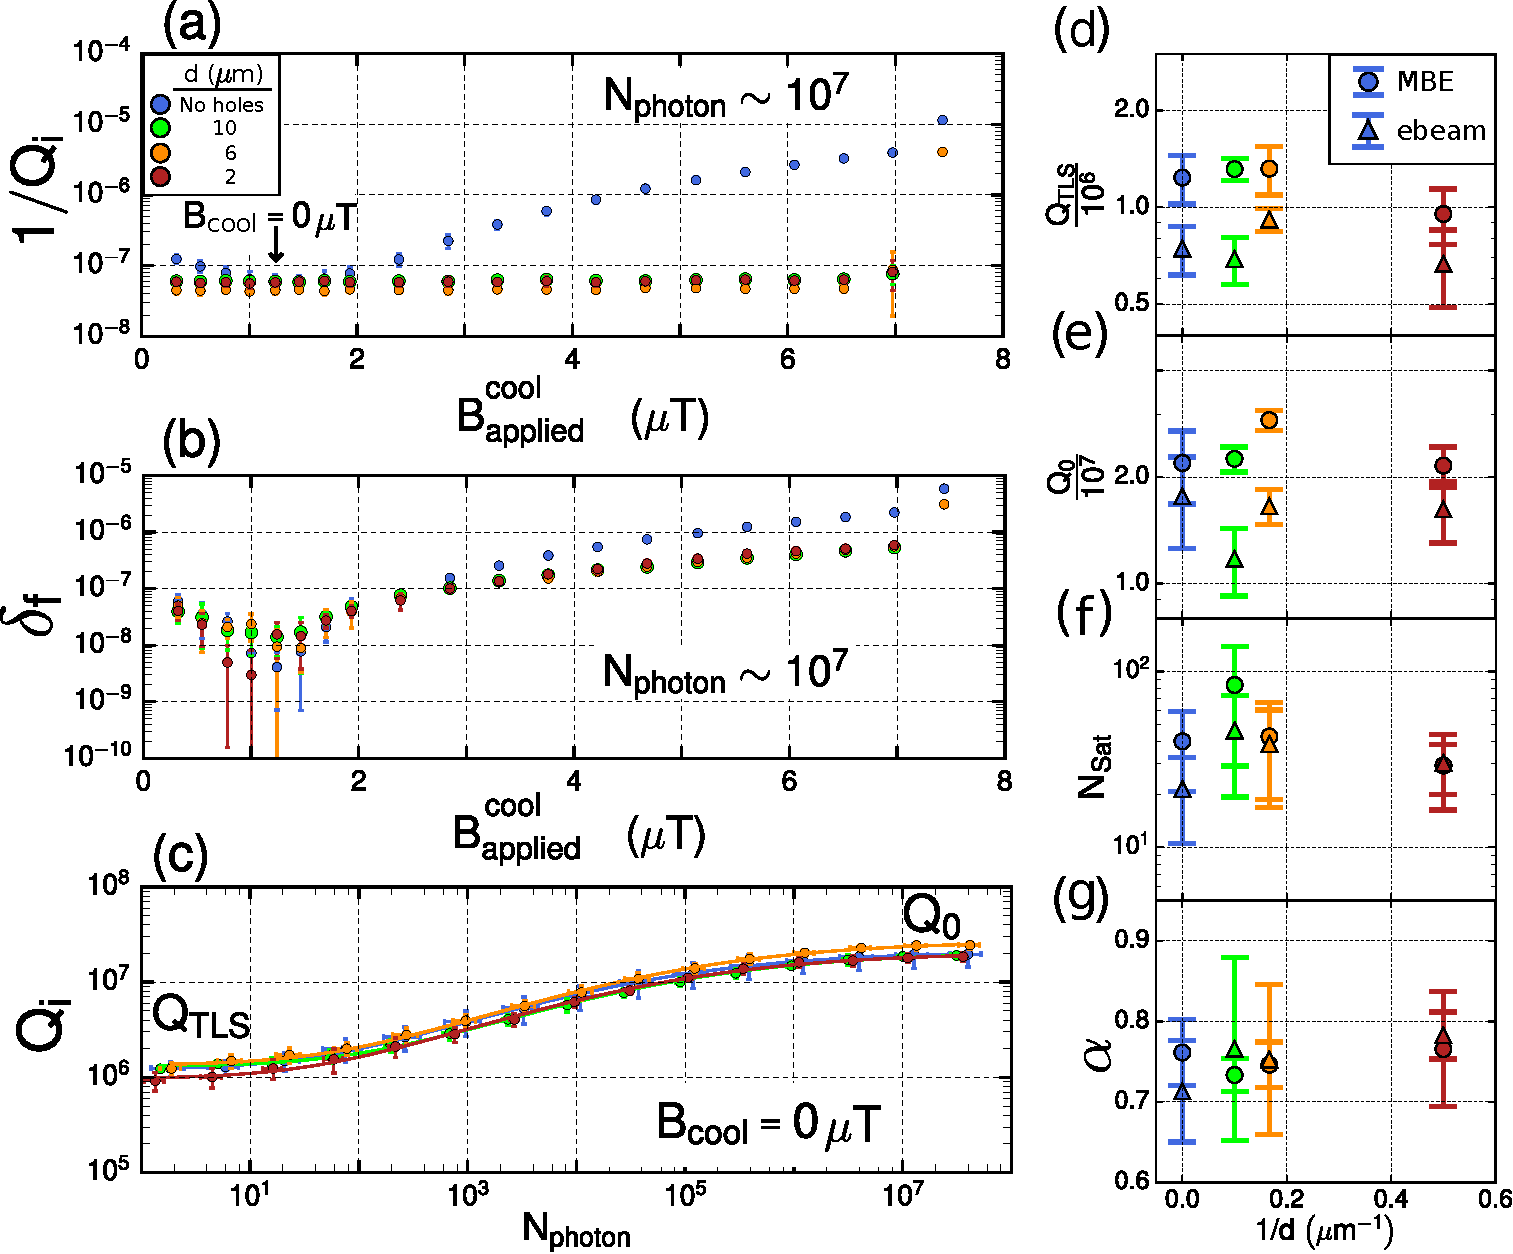
\includegraphics[width=500 pt]{DielectricFluxTrap_ExpData_arxiv_Rev2c_proof_revision1.pdf}
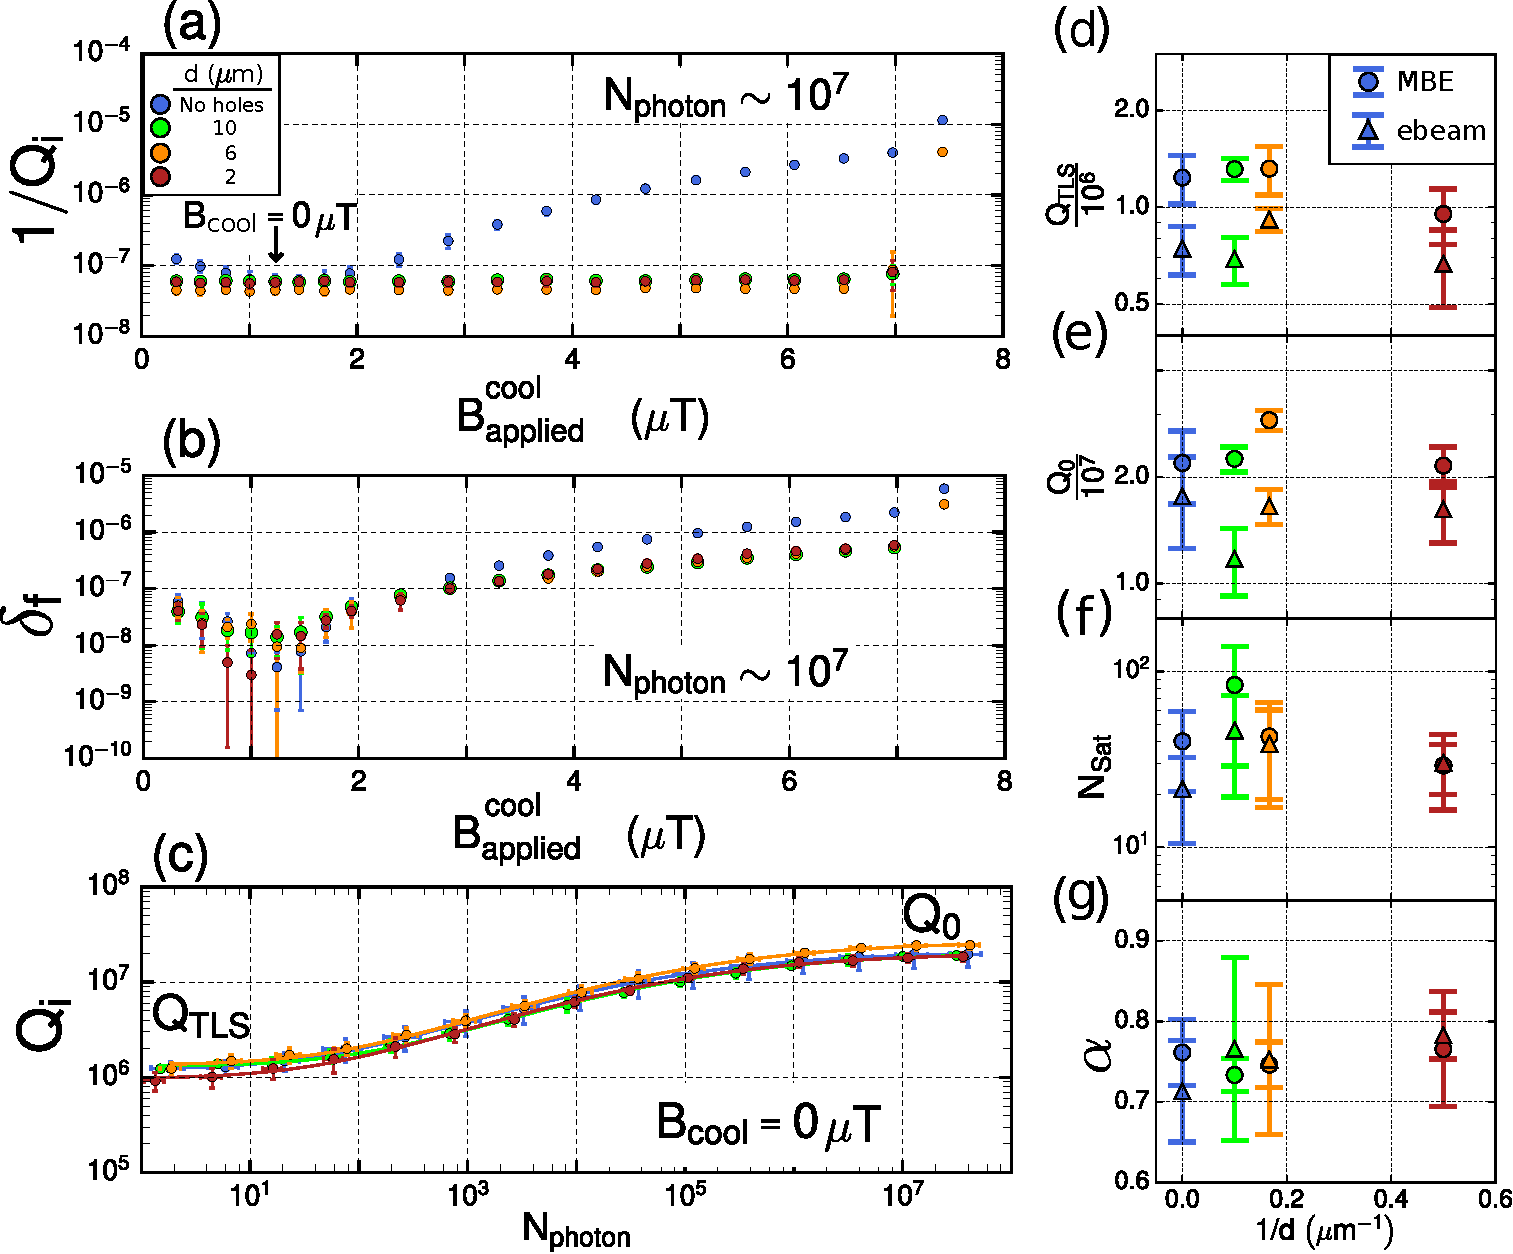
\includegraphics[width=400 pt]{DielectricFluxTrap_ExpData_arxiv_Rev2c_proof_revision1.pdf}

\end{center}
\caption{(Color) Measurement results  (a) and (b) Loss $1/Q_i$ and resonator fractional frequency shift $\delta_{\textrm{f}}$ versus applied magnetic field when cooled through $T_c$ $\Bcapp$, taken at high power $N_\textrm{photon} \sim 10^7$.  Data is for the MBE-grown film and hole patterns of varying density.  The resonators with no holes have the greatest sensitivity to magnetic fields, so the minimum of loss identifies the true zero giving the cryostat offset field.  (c) The dependence of $Q_i$ on measurement drive power for the MBE sample, fit to a standard TLS dissipation model from Eqn.\,\ref{TLS_dissipation}.  (d) - (g) Extracted TLS model parameters from power dependence measurements as shown in (c) for the MBE and e-beam samples, showing loss attributed to unsaturated TLS (low power) and due to power independent mechanisms (high power) vs the edge to edge hole spacing d.  In all plots the data shows mean value for resonators of a common hole density, with error bars indicating 1 standard deviation.}
\label{Resonator Measurements}
\end{figure*}

The loss is determined by measuring the resonator intrinsic quality factor $Q_i$ using transmission spectroscopy\cite{megrant2012}.  In the initial measurement phase, we measure $Q_i$ versus applied magnetic field at high power for better signal to noise ratio, since vortex loss has weak power dependence\cite{bothner2011}.  To vary $B_\textrm{cool}$, we raise the device temperature above $\text{T}_{c}$, set the applied magnetic field $\Bcapp$, and cool the sample back through its $\text{T}_{c}$ in this field thereby trapping magnetic vortices.  Once the device has returned to its base temperature we extract the resonator $Q_i$ from $S_{21}$ measurements with a vector network analyzer (VNA).

Figure\,\ref{Resonator Measurements} (a) shows the magnetic field dependence of $Q_i$ for resonators with and without ground plane holes from the MBE device.  For resonators without a patterned ground plane there is a well defined maximum of $Q_i$ that identifies the applied field that zeros the total magnetic field.\cite{chiaro2015supp}  The offset between $\Bcapp$ and $B_{\textrm{cool}}$ is indicated by the arrow.  We observe a gradual but significant increase in loss away from this field that is attributed to a greater density of magnetic vortices trapped in the ground plane.  As expected, for resonators with holes we find that $Q_i$ is nearly independent of applied magnetic field until the critical field for vortex formation in the center trace has been exceeded.  Figure\,\ref{Resonator Measurements} (b) shows the fractional frequency shift  \mbox{$\delta_{\text{f}}=( f_{0}(\Bcapp=0) - f_0(\Bcapp))/f_{0}(\Bcapp=0)$} we observe that resonators with patterned ground planes are less susceptible to field induced frequency shifts.

For MBE grown resonators with hole patterns we consider data in the field range of $\Bcapp=1.4-6.4$\,$\mu\text{T}$.  Fields in this range are less than the critical field for vortex formation in the center trace of the resonator and allows us to estimate the residual magnetic loss in the absence of local magnetic vortices.  By assuming an excess loss model that is linear in $\Bcapp$, we estimate the residual magnetic loss to be \mbox{$8.6 \pm 1.3 \times 10^{-10}$\,/$\mu\text{T}$.}  We show the data supporting this estimate in the supplement.\cite{chiaro2015supp}  Although additional experiments are required to determine the origin and proper functional dependence of this excess loss, we suggest likely models are coupling to vortices in remote areas of the device not protected by the hole overlays or quasiparticles generated by the local suppression of $T_c$ due to the magnetic field.  For typical shielded devices, this estimate is several orders of magnitude below the loss of the best SCPW resonators.\cite{megrant2012, ohya2013, bruno2015}

After measuring the magnetic field dependence of the high power $Q_i$ we quantify the surface loss from TLS defects by measuring the power dependence of the resonator $Q_i$.  We use the value of $\Bcapp$ that maximizes $Q_i$ at high power, so that $B_{\text{cool}} = 0\,\mu\text{T}$ as described previously.  The power dependence data for the MBE device is shown in Fig.\,\ref{Resonator Measurements}(c), where the lines are fits to a standard TLS loss model \cite{wang2009}
\begin{equation}
\label{TLS_dissipation}
\frac{1}{Q_i} = \frac{1}{Q_\text{TLS}}\frac{1}{\sqrt{1+\left( \frac{N_\text{photon}} {N_\text{sat}}\right)^\alpha}} + \frac{1}{Q_0}
\end{equation}
This model decomposes the total internal loss of the resonator $1/Q_i$ into a power independent loss term $1/Q_0$ that includes such loss modes from quasiparticles and radiation, and a power dependent term of magnitude $1/Q_\text{TLS}$ that comes from TLS defects.  Here $N_\text{photon}$ is the excitation number of photons in the resonator and $N_\text{sat}$ describes the saturation field of the TLS bath.  The parameter $\alpha$ is related to the electric field distribution of the resonator, and may be influenced by interactions between TLS defects within the bath.\cite{faoro2012, faoro2015}

Figure \ref{Resonator Measurements}(d) and (e) show the quality factors for the low power ($Q_\textrm{TLS}$) and high power ($Q_0$) regimes, extracted from the fits in (c).  The data points represent resonators from two circuits from each film.  In (d), we see that the densest hole pattern increases TLS loss by roughly 25\% relative to resonators without holes for both the MBE and ebeam grown resonators.  Dielectric TLS loss is often decomposed as \mbox{$\Qtlsparticipation$} where \mbox{$\tan \delta_i$} is the loss tangent of dielectric volume $i$ and the participation ratio $p_i$ is the fraction of the electric energy of the resonator excitation that is stored within that volume.\cite{wang2015, barends2010, gao2008}  We presume that the increase in TLS loss is not due to an increase in the dielectric loss tangent, but rather due to an increase in the participation ratio resulting from a redistribution of the electric field.

To quantify the excess loss due to the dense hole pattern we perform linear regression analysis controlling for the difference between the MBE and ebeam films.\cite{chiaro2015supp}  This analysis includes the results from 23 resonators, 11 measured on two circuits from the MBE film and 12 measured on two circuits from the ebeam film.  We find that the TLS loss $1/Q_\text{TLS}$ directly attributable to the dense hole pattern is $2.5 \pm 1.3\times 10^{-7}$, where the uncertainty represents the standard error.  The p-value for this regression coefficient is 0.07.

When using the resonators for quantum devices at low magnetic fields, this increase in loss is undesirable.  The hole spacing should thus be carefully chosen, first to be close enough to provide protection from external fields of magnitude $\sim \Phi_0/d^2$, where $d$ is the edge to edge spacing between holes\cite{stan2004}.  However, the spacing from the resonator to the first row of holes should be greater than about $6\,\mu\textrm{m}$, a value that did not exhibit measurable excess TLS loss.  In (e) we observe that the $Q_0$ of resonators with the densest hole pattern is nearly the same as that without any hole overlay.  This indicates that power independent loss mechanisms were not affected by the hole patterns.

We have characterized dissipation from arrays of flux-trapping holes in SCPW resonators.  We find that excess dielectric loss can be made vanishingly small by increasing the distance between the resonator edge and the array.  In our experiment, a 6\,$\mu \text{m}$ separation was enough to remove excess dielectric loss; power-independent loss mechanisms were not affected by the arrays.  We also estimate the residual magnetic loss in resonators with ground plane holes to be $\sim$\,$10^{-9}$\,/$\mu\text{T}$, showing that SCPW resonators can be made insensitive to small magnetic fields without magnifying other loss mechanisms.

\draftcomment{
\section*{ACKNOWLEDGEMENTS}%
Devices were fabricated at the UCSB Nanofabrication Facility, a part of the NSF-funded National Nanotechnology Infrastructure Network.  This research was funded by the Office of the Director of National Intelligence (ODNI), Intelligence Advanced Research Projects Activity (IARPA), through Army Research Office Grant No. W911NF-09-1-0375 and by Google Inc. All statements of fact, opinion, or conclusions contained herein are those of the authors and should not be construed as representing the official views or policies of IARPA, the ODNI, the U.S. Government.
}

\clearpage
%\end{document}






